\documentclass[plain]{beamer}
\setbeamertemplate{navigation symbols}{}
\setbeamercolor{frametitle}{fg=black}
\setbeamercolor{title}{fg=black}

\usepackage[ngerman]{babel}
\usepackage{graphics}
\usepackage{minted}
\usepackage{xcolor}

\newcommand{\cpp}{\texttt{C++}}
\newcommand{\demoslide}{\begin{frame}
  \center \huge DEMO
\end{frame}}

\title{\huge \cpp{}}
\author{Max Schik}

\begin{document}
\begin{frame}
  \titlepage
\end{frame}

\begin{frame}
  \frametitle{Einleitung}
  \begin{columns}[onlytextwidth,T]
    \column{\dimexpr\linewidth-50mm-5mm}
    \begin{itemize}
      \item Aus dem Jahre 1985 (38 Jahre alt)
      \item Entwickelt von Bjarne Stroustrup
      \item Fing an als C mit Klassen, hat aber heute nur noch wenig mit C zu tun
    \end{itemize}
    \column{50mm}
    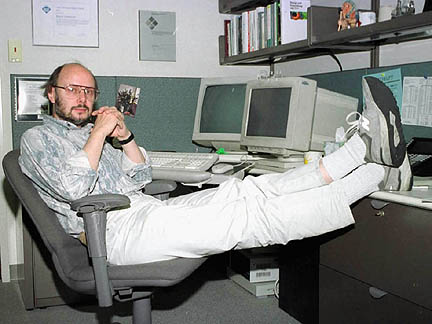
\includegraphics[width=\textwidth]{imgs/BjarneStroustrup.jpg}
  \end{columns}
\end{frame}

\begin{frame}
  \frametitle{Einleitung}
  \begin{itemize}
    \item Sehr, sehr, sehr viele Features für eine Sprache
    \item Das hier ist nur ein minimaler Einblick (ich hab nur 30min)
    \item Wichtigste Skills: Dokumentation lesen
  \end{itemize}
  \center 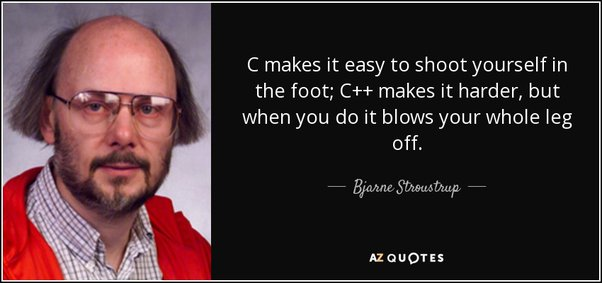
\includegraphics[height=0.4\textheight]{imgs/no-leg.jpeg}
\end{frame}

\begin{frame}
  \center \huge Grundlegenes
\end{frame}

\begin{frame}[fragile]
  \frametitle{Ein erstes "Hello World"}
  \inputminted{cpp}{code/examples/helloworld.cpp}
  \begin{itemize}
    \item Kompilieren mit \texttt{g++ helloworld.cpp -o helloworld}
    \item In ROS Projekten wird das von \texttt{catkin\_make} übernommen
  \end{itemize}
\end{frame}

\begin{frame}[fragile]
  \frametitle{Grundlegene Typen}
  \inputminted{cpp}{code/examples/types.cpp}
\end{frame}

\begin{frame}[fragile]
  \frametitle{Kontrollfluss}
  \inputminted{cpp}{code/examples/fizzbuzz.cpp}
\end{frame}

\begin{frame}[fragile]
  \frametitle{Funktionen}
  \inputminted{cpp}{code/examples/functions.cpp}
\end{frame}

\begin{frame}[fragile]
  \frametitle{Klassen und Structs}
  \inputminted{cpp}{code/examples/classes.cpp}
\end{frame}

\begin{frame}[fragile]
  \frametitle{Klassen und Structs}
  \begin{columns}[onlytextwidth,T]
    \column{\dimexpr\linewidth-50mm-10mm}
    \inputminted{cpp}{code/examples/structs.cpp}
    \column{50mm}
    \begin{itemize}
      \item Member von Klassen sind per default \texttt{private}
      \item Member von Structs sind per default \texttt{public}
      \item Wenn es nur darum geht Daten zu speichern sollte man Structs verwenden, ansonsten
        Klassen
    \end{itemize}
  \end{columns}
\end{frame}


\begin{frame}
  \center \huge Unterschiede zu 'moderneren' Sprachen
\end{frame}

\begin{frame}
  \frametitle{Headerfiles}
  \begin{itemize}
    \item Module/Bibliotheken werden mit \texttt{\#include} importiert
    \item Dafür wird in die \emph{Deklaration} in den Header geschrieben und die \emph{Definition}
      in eine andere Datei
      \begin{itemize}
        \item \textbf{Deklaration:} Wie heißt die Funktion, welche Argumente nimmt sie an und was
          gibt sie zurück
        \item \textbf{Definition:} Die eigentliche Implementation der Funktion
      \end{itemize}
  \end{itemize}
\end{frame}


\begin{frame}
  \frametitle{Headerfiles}
  \begin{columns}[onlytextwidth,T]
    \column{\dimexpr0.5\linewidth}
    \texttt{lib.h} (\emph{Deklaration}):
    \inputminted{cpp}{code/examples/lib.h}
    \vspace{5mm}
    \texttt{lib.cpp} (\emph{Defintion}):
    \inputminted{cpp}{code/examples/lib.cpp}
    \column{\dimexpr0.5\linewidth}
    \texttt{lib\_main.cpp:}
    \inputminted{cpp}{code/examples/lib_main.cpp}
  \end{columns}
\end{frame}


\begin{frame}
  \frametitle{Pass By Value}
  \begin{itemize}
    \item In \cpp{} ist alles ist pass-by-value
    \item Argumente für Funktionen etc. werden kopiert (auch Objekte)
    \item Vergleich: In Java sind Objekte pass-by-reference
  \end{itemize}
\end{frame}

\begin{frame}[fragile]
  \frametitle{Pointer}
  \begin{columns}
    \column{\dimexpr0.4\linewidth}
    \inputminted[firstline=0, lastline=17]{cpp}{code/examples/pointer.cpp}
    \column{\dimexpr0.6\linewidth}
    \begin{itemize}
      \item Ein Pointer 'zeigt' auf den Speicherbereich einer anderen 'Variabel'
      \item Problematisch weil sich der Entwickler selber um seinen Speicher kümmern muss
      \item \textit{ich mag sie nicht und finde man sollte sie nach möglichkeit nicht verwenden}
      \item Lösung in modernem \cpp{}: Referenzen und \texttt{shared\_ptr}
    \end{itemize}
  \end{columns}
\end{frame}

\begin{frame}
  \frametitle{Pointer}
  \center 
\includegraphics[height=0.8\textheight]{imgs/pointer_meme.png}
\end{frame}

\begin{frame}[fragile]
  \frametitle{Pass By Value}
  \begin{columns}
    \column{\dimexpr0.4\linewidth}
    \inputminted[firstline=0, lastline=17]{cpp}{code/examples/passbyvalue.cpp}
    \column{\dimexpr0.6\linewidth}
    \inputminted[firstline=19]{cpp}{code/examples/passbyvalue.cpp}
  \end{columns}
\end{frame}

\demoslide{}

\begin{frame}
  \frametitle{In case of Error}
  \begin{itemize}
    \item Sehr, sehr lange unverständliche Fehlermeldung \textrightarrow{} vermutlich was mit
      Templates (wenn man den Typ mit angibt, z. Bsp \texttt{std::vector<int>}) oder Typ fehler.
    \item Segmentation Fault \textrightarrow{} vermutlich 'illegalen' Speicher verwendet, z. Bsp
      \texttt{nullptr}
    \item Der Linker (\texttt{ld}) schlägt fehl \textrightarrow{} vermutlich fehlt von einer
      Funktion oder so die Definition
  \end{itemize}
\end{frame}

\begin{frame}
  \frametitle{Und jetzt?}
  \begin{itemize}
    \item Morgen findet der Advanced \cpp{} Workshop von Noah statt
    \item \url{https://en.cppreference.com/w/}
    \item \url{https://isocpp.github.io/CppCoreGuidelines/CppCoreGuidelines}
    \item \url{http://wiki.ros.org/ROS/Tutorials/WritingPublisherSubscriber\%28c\%2B\%2B\%29}
  \end{itemize}
\end{frame}

\begin{frame}
  \frametitle{Viel Spaß beim Programmieren}
  \center 
\includegraphics[width=0.9\textwidth]{imgs/error-messages.png}
\end{frame}


\end{document}
